\title{计数原理（2016--2025 高考真题）}
\author{}
\date{}
\maketitle
\noindent 本专题共 44 道题，按年份排列。每题标注原卷与原题号。

\section*{2016 年}

\begin{question}[points=5]
\textbf{来源：}2016 年 全国III卷-理科，第 7 题\par
执行如图程序框图, 如果输入的 $a=4$, $b=6$, 那么输出的 $n=$

\begin{center}
  
\includegraphics[width=.42\linewidth]{assets/asset-001-01.jpg}
\end{center}
\begin{choices}
  \item $3$
  \item $4$
  \item $5$
  \item $6$
\end{choices}
\begin{solution}
\textbf{答案：}$4$

\textbf{分析：}模拟执行程序, 根据赋值语句的功能依次写出每次循环得到的 $a,b,s,n$ 的值, 当 $s=20$ 时满足条件 $s>16$, 退出循环.

\textbf{详解：}模拟执行程序, 可得 $a=4,b=6,n=0,s=0$; 执行循环体, $a=2,b=4,a=6,s=6,n=1$; 不满足条件 $s>16$, 执行循环体, $a=-2,b=6,a=4,s=10,n=2$; 不满足条件 $s>16$, 执行循环体, $a=2,b=4,a=6,s=16,n=3$; 不满足条件 $s>16$, 执行循环体, $a=-2,b=6,a=4,s=20,n=4$; 满足条件 $s>16$, 退出循环, 输出 $n=4$, 故选 B.
\end{solution}
\end{question}

\begin{question}[points=5]
\textbf{来源：}2016 年 全国III卷-理科，第 12 题\par
定义 "规范 $01$ 数列" $\{a_n\}$ 如下: $\{a_n\}$ 共有 $2m$ 项, 其中 $m$ 项为 $0$, $m$ 项为 $1$, 且对任意 $k\le 2m$, $a_1,a_2,\dots,a_k$ 中 $0$ 的个数不少于 $1$ 的个数, 若 $m=4$, 则不同的 "规范 $01$ 数列" 共有
\begin{choices}
  \item $18$ 个
  \item $16$ 个
  \item $14$ 个
  \item $12$ 个
\end{choices}
\begin{solution}
\textbf{答案：}$14$ 个

\textbf{分析：}由新定义可得, "规范 $01$ 数列" 有偶数项 $2m$ 项, 且所含 $0$ 与 $1$ 的个数相等, 首项为 $0$, 末项为 $1$, 当 $m=4$ 时, 数列中有四个 $0$ 和四个 $1$, 然后一一列举得答案.

\textbf{详解：}由题意可知, 数列有 $8$ 项, 满足条件的数列有: $0,0,0,0,1,1,1,1$; $0,0,0,1,0,1,1,1$; $0,0,0,1,1,0,1,1$; $0,0,0,1,1,1,0,1$; $0,0,1,0,0,1,1,1$; $0,0,1,0,1,0,1,1$; $0,0,1,0,1,1,0,1$; $0,0,1,1,0,1,0,1$; $0,0,1,1,0,0,1,1$; $0,1,0,0,0,1,1,1$; $0,1,0,0,1,0,1,1$; $0,1,0,0,1,1,0,1$; $0,1,0,1,0,0,1,1$; $0,1,0,1,0,1,0,1$. 共 $14$ 个, 故选 C.
\end{solution}
\end{question}

\begin{question}[points=5]
\textbf{来源：}2016 年 全国III卷-文科，第 8 题\par
执行如图程序框图, 如果输入的 $a=4$, $b=6$, 那么输出的 $n=$ ( )

\begin{center}
  
\includegraphics[width=.42\linewidth]{assets/asset-003-01.jpg}
\end{center}
\begin{choices}
  \item $3$
  \item $4$
  \item $5$
  \item $6$
\end{choices}
\begin{solution}
\textbf{答案：}$4$

\textbf{分析：}模拟执行程序, 根据赋值语句的功能依次写出每次循环得到的 $a,b,s,n$ 的值, 当 $s=20$ 时满足条件 $s>16$, 退出循环, 输出 $n$ 的值为 $4$.

\textbf{详解：}模拟执行程序, 可得 $a=4,b=6,n=0,s=0$; 执行循环体, $a=2,b=4,a=6,s=6,n=1$; 不满足条件 $s>16$, 执行循环体, $a=-2,b=6,a=4,s=10,n=2$; 不满足条件 $s>16$, 执行循环体, $a=2,b=4,a=6,s=16,n=3$; 不满足条件 $s>16$, 执行循环体, $a=-2,b=6,a=4,s=20,n=4$; 满足条件 $s>16$, 退出循环, 输出 $n$ 的值为 $4$. 故选 B.
\end{solution}
\end{question}

\begin{question}[points=5]
\textbf{来源：}2016 年 全国II卷-理科，第 5 题\par
如图，小明从街道的$E$处出发，先到$F$处与小红会合，再一起到位于$G$处的老年公寓参加志愿者活动，则小明到老年公寓可以选择的最短路径条数为（\quad）

\begin{center}
  
\includegraphics[width=.42\linewidth]{assets/asset-004-01.jpg}
\end{center}
\begin{choices}
  \item $24$
  \item $18$
  \item $12$
  \item $9$
\end{choices}
\begin{solution}
\textbf{答案：}$18$

\textbf{分析：}从$E$到$F$最短的走法，无论怎样走，一定包括$4$段，其中$2$段方向相同，另$2$段方向相同，每种最短走法，即是从$4$段中选出$2$段走东向的，选出$2$段走北向的，由组合数可得最短的走法，同理从$F$到$G$，最短的走法，有$C_3^1=3$种走法，利用乘法原理可得结论．

\textbf{详解：}从$E$到$F$有$C_4^2C_2^2=6$种走法，从$F$到$G$有$C_3^1C_2^2=3$种走法，故总路径条数为$6\times3=18$．故选B．
\end{solution}
\end{question}

\begin{question}[points=5]
\textbf{来源：}2016 年 全国II卷-理科，第 8 题\par
中国古代有计算多项式值的秦九韶算法，如图是实现该算法的程序框图．执行该程序框图，若输入的$x=2$，$n=2$，依次输入的$a$为$2$，$2$，$5$，则输出的$s=$（\quad）

\begin{center}
  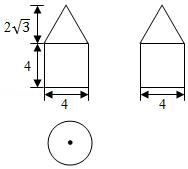
\includegraphics[width=.42\linewidth]{assets/asset-005-01.jpg}
\end{center}
\begin{choices}
  \item $7$
  \item $12$
  \item $17$
  \item $34$
\end{choices}
\begin{solution}
\textbf{答案：}$17$

\textbf{分析：}根据已知的程序框图可得，该程序的功能是利用循环结构计算并输出变量S的值，模拟程序的运行过程，可得答案．

\textbf{详解：}模拟运行：输入$x=2,n=2$；第一次输入$a=2$，$s=2$，$k=1$；第二次输入$a=2$，$s=6$，$k=2$；第三次输入$a=5$，$s=17$，$k=3$，满足$k>n$，输出$s=17$．故选C．
\end{solution}
\end{question}

\begin{question}[points=5]
\textbf{来源：}2016 年 全国II卷-理科，第 15 题\par
有三张卡片，分别写有$1$和$2$，$1$和$3$，$2$和$3$．甲，乙，丙三人各取走一张卡片，甲看了乙的卡片后说：“我与乙的卡片上相同的数字不是$2$”，乙看了丙的卡片后说：“我与丙的卡片上相同的数字不是$1$”，丙说：“我的卡片上的数字之和不是$5$”，则甲的卡片上的数字是．
\fillin[{$1$和$3$}]
\begin{solution}
\textbf{答案：}$1$和$3$

\textbf{分析：}可先根据丙的说法推出丙的卡片上写着$1$和$2$，或$1$和$3$，分别讨论这两种情况，根据甲和乙的说法可分别推出甲和乙卡片上的数字，这样便可判断出甲卡片上的数字是多少．

\textbf{详解：}若丙的卡片是$1$和$2$，则乙的卡片是$2$和$3$，甲的卡片是$1$和$3$（符合甲的说法）；若丙的卡片是$1$和$3$，则乙的卡片是$2$和$3$，此时甲说与乙相同的数字不是$2$，则甲只能是$1$和$2$，但$1$和$2$的卡片不存在，矛盾．故甲的是$1$和$3$．
\end{solution}
\end{question}

\begin{question}[points=5]
\textbf{来源：}2016 年 全国I卷-理科，第 14 题\par
$(2x+\sqrt{x})^5$的展开式中，$x^3$的系数是．（用数字填写答案）
\fillin[{$10$}]
\begin{solution}
\textbf{答案：}$10$

\textbf{分析：}利用二项展开式的通项公式求出第$r+1$项，令$x$的指数为$3$，求出$r$，即可求出展开式中$x^3$的系数．

\textbf{详解：}解：$(2x+\sqrt{x})^5$的展开式中，通项公式为：$T_{r+1}=C_5^r(2x)^{5-r}(\sqrt{x})^r=2^{5-r}C_5^r x^{5-\frac{r}{2}}$，令$5-\frac{r}{2}=3$，解得$r=4$，所以$x^3$的系数$2^{1}C_5^4=10$．故答案为：$10$．
\end{solution}
\end{question}

\section*{2017 年}

\begin{question}[points=5]
\textbf{来源：}2017 年 全国III卷-理科，第 4 题\par
$(x+y)(2x-y)^5$的展开式中的$x^3y^3$系数为（ ）
\begin{choices}
  \item $-80$
  \item $-40$
  \item $40$
  \item $80$
\end{choices}
\begin{solution}
\textbf{答案：}$C$

\textbf{分析：}$(2x-y)^5$的展开式的通项公式：$T_{r+1}=C_{5}^{r}(2x)^{5-r}(-y)^r=2^{5-r}(-1)^r C_{5}^{r}x^{5-r}y^r$。令$5-r=2$，$r=3$，解得$r=3$。令$5-r=3$，$r=2$，解得$r=2$。即可得出。

\textbf{详解：}$(2x-y)^5$的展开式的通项公式：$T_{r+1}=C_{5}^{r}(2x)^{5-r}(-y)^r=2^{5-r}(-1)^r C_{5}^{r}x^{5-r}y^r$。令$5-r=2$，$r=3$，解得$r=3$。令$5-r=3$，$r=2$，解得$r=2$。所以$(x+y)(2x-y)^5$的展开式中的$x^3y^3$系数$=2^2\times(-1)^3 C_{5}^{3}+2^3\times C_{5}^{2}=40$。故选C。
\end{solution}
\end{question}

\begin{question}[points=5]
\textbf{来源：}2017 年 全国II卷-理科，第 6 题\par
安排 $3$ 名志愿者完成 $4$ 项工作，每人至少完成 $1$ 项，每项工作由 $1$ 人完成，则不同的安排方式共有（   ）
\begin{choices}
  \item $12$ 种
  \item $18$ 种
  \item $24$ 种
  \item $36$ 种
\end{choices}
\begin{solution}
\textbf{答案：}$D$

\textbf{分析：}把工作分成 $3$ 组，然后安排工作方式即可。

\textbf{详解：}$4$ 项工作分成 $3$ 组，可得：$C_4^2=6$，安排 $3$ 名志愿者完成 $4$ 项工作，每人至少完成 $1$ 项，每项工作由 $1$ 人完成，可得：$6\times A_3^3=36$ 种．故选：$D$。
\end{solution}
\end{question}

\begin{question}[points=5]
\textbf{来源：}2017 年 全国I卷-理科，第 6 题\par
$(1+\frac{1}{x^2})(1+x)^6$ 展开式中 $x^2$ 的系数为（ ）
\begin{choices}
  \item $15$
  \item $20$
  \item $30$
  \item $35$
\end{choices}
\begin{solution}
\textbf{答案：}C

\textbf{分析：}直接利用二项式定理的通项公式求解即可．

\textbf{详解：}$(1+\frac{1}{x^2})(1+x)^6$ 展开式中：若 $(1+\frac{1}{x^2})$ 提供常数项 1，则 $(1+x)^6$ 提供含有 $x^2$ 的项，可得展开式中 $x^2$ 的系数：$C_6^2=15$；若 $(1+\frac{1}{x^2})$ 提供 $x^{-2}$ 项，则 $(1+x)^6$ 提供含有 $x^4$ 的项，可得展开式中 $x^2$ 的系数：$C_6^4=15$．故 $(1+\frac{1}{x^2})(1+x)^6$ 展开式中 $x^2$ 的系数为：$15+15=30$．故选：C．
\end{solution}
\end{question}

\section*{2018 年}

\begin{question}[points=5]
\textbf{来源：}2018 年 全国III卷-理科，第 5 题\par
$(x^2+\frac{2}{x})^5$的展开式中$x^4$的系数为（ ）
\begin{choices}
  \item $10$
  \item $20$
  \item $40$
  \item $80$
\end{choices}
\begin{solution}
\textbf{答案：}C

\textbf{分析：}由二项式定理得展开式的通项，令指数为4求得$r$，再求系数．

\textbf{详解：}由二项式定理得$(x^2+\frac{2}{x})^5$的展开式的通项为：$T_{r+1}=C_5^r (x^2)^{5-r}(\frac{2}{x})^r=2^r C_5^r x^{10-3r}$，由$10-3r=4$，解得$r=2$，$\therefore$系数为$2^2 C_5^2=4\times10=40$．
\end{solution}
\end{question}

\begin{question}[points=5]
\textbf{来源：}2018 年 全国I卷-理科，第 15 题\par
从2位女生，4位男生中选3人参加科技比赛，且至少有1位女生入选，则不同的选法共有种。（用数字填写答案）
\fillin[{$16$}]
\begin{solution}
\textbf{答案：}$16$

\textbf{分析：}方法一：直接法，分类即可求出；方法二：间接法，先求出没有限制的种数，再排除全是男生的种数。

\textbf{详解：}方法一（直接法）：1女2男，有$C_2^1C_4^2=12$种；2女1男，有$C_2^2C_4^1=4$种，所以共有$12+4=16$种。
方法二（间接法）：$C_6^3-C_4^3=20-4=16$种。
\end{solution}
\end{question}

\section*{2019 年}

\begin{question}[points=5]
\textbf{来源：}2019 年 全国III卷-理科，第 4 题\par
$(1+2x^2)(1+x)^4$ 的展开式中 $x^3$ 的系数为
\begin{choices}
  \item $12$
  \item $16$
  \item $20$
  \item $24$
\end{choices}
\begin{solution}
\textbf{答案：}A

\textbf{分析：}本题利用二项展开式通项公式求展开式指定项的系数。

\textbf{详解：}由题意得 $x^3$ 的系数为 $C_4^3 + 2C_4^1 = 4 + 8 = 12$。故选 A。
\end{solution}
\end{question}

\section*{2020 年}

\begin{question}[points=5]
\textbf{来源：}2020 年 全国III卷-理科，第 14 题\par
$\left(x^2+\dfrac{2}{x}\right)^6$ 的展开式中常数项是 （用数字作答）。
\fillin[{$240$}]
\begin{solution}
\textbf{答案：}$240$

\textbf{分析：}写出二项展开式通项，令 $x$ 的指数为零求得 $r$ 再计算。

\textbf{详解：}$T_{r+1}=C_6^r(x^2)^{6-r}\cdot\left(\dfrac{2}{x}\right)^r=C_6^r 2^r x^{12-3r}$，令 $12-3r=0$，得 $r=4$。常数项为 $C_6^4 2^4=15\times16=240$。
\end{solution}
\end{question}

\begin{question}[points=5]
\textbf{来源：}2020 年 全国II卷-理科，第 14 题\par
4名同学到3个小区参加垃圾分类宣传活动，每名同学只去1个小区，每个小区至少安排1名同学，则不同的安排方法共有种.
\fillin[{$36$}]
\begin{solution}
\textbf{答案：}$36$

\textbf{分析：}根据题意，采用捆绑法，先取2名同学看作一组，现在可看成是3组同学分配到3个小区，即可求得答案.

\textbf{详解：}$\because$4名同学到3个小区参加垃圾分类宣传活动，每名同学只去1个小区，每个小区至少安排1名同学，$\therefore$先取2名同学看作一组，选法有$\mathrm{C}_4^2=6$，现在可看成是3组同学分配到3个小区，分法有$\mathrm{A}_3^3=6$，根据分步乘法原理，可得不同的安排方法$6\times6=36$种.
\end{solution}
\end{question}

\begin{question}[points=5]
\textbf{来源：}2020 年 全国II卷-文科，第 3 题\par
如图，将钢琴上的12个键依次记为 $a_1, a_2, \ldots, a_{12}$。设 $1\le i<j<k\le 12$。若 $k-j=3$ 且 $j-i=4$，则称 $a_i, a_j, a_k$ 为原位大三和弦；若 $k-j=4$ 且 $j-i=3$，则称 $a_i, a_j, a_k$ 为原位小三和弦。用这12个键可以构成的原位大三和弦与原位小三和弦的个数之和为（ ）

\begin{center}
  
\includegraphics[width=.42\linewidth]{assets/asset-016-01.jpg}
\end{center}
\begin{choices}
  \item $5$
  \item $8$
  \item $10$
  \item $15$
\end{choices}
\begin{solution}
\textbf{答案：}C

\textbf{分析：}根据原位大三和弦满足 $k-j=3, j-i=4$，原位小三和弦满足 $k-j=4, j-i=3$，从 $i=1$ 开始，利用列举法即可解出。

\textbf{详解：}原位大三和弦满足：$k-j=3, j-i=4$。
$i=1, j=5, k=8$；$i=2, j=6, k=9$；$i=3, j=7, k=10$；$i=4, j=8, k=11$；$i=5, j=9, k=12$。
原位小三和弦满足：$k-j=4, j-i=3$。
$i=1, j=4, k=8$；$i=2, j=5, k=9$；$i=3, j=6, k=10$；$i=4, j=7, k=11$；$i=5, j=8, k=12$。
故个数之和为10。
故选：C。
\end{solution}
\end{question}

\begin{question}[points=5]
\textbf{来源：}2020 年 全国I卷-理科，第 8 题\par
$\left(x+\frac{y^2}{x}\right)(x+y)^5$的展开式中$x^3y^3$的系数为
\begin{choices}
  \item $5$
  \item $10$
  \item $15$
  \item $20$
\end{choices}
\begin{solution}
\textbf{答案：}C

\textbf{详解：}$(x+y)^5$展开式的通项$T_{r+1}=C_5^r x^{5-r}y^r$。$x\cdot T_{r+1}=C_5^r x^{6-r}y^r$，令$r=3$得$x^3y^3$系数$C_5^3=10$；$\frac{y^2}{x}\cdot T_{r+1}=C_5^r x^{4-r}y^{r+2}$，令$r=1$得$x^3y^3$系数$C_5^1=5$。故系数为$10+5=15$。
\end{solution}
\end{question}

\section*{2021 年}

\begin{question}[points=5]
\textbf{来源：}2021 年 北京卷，第 11 题\par
$(x^3-\frac{1}{x})^4$ 展开式中常数项为.
\fillin[{$-4$}]
\begin{solution}
\textbf{答案：}$-4$

\textbf{详解：}$(x^3-\frac{1}{x})^4$ 的展开式的通项 $T_{r+1}=C_4^r (x^3)^{4-r}(-\frac{1}{x})^r=(-1)^r C_4^r x^{12-4r}$, 令 $r=3$ 得常数项为 $T_4=(-1)^3 C_4^3=-4$.
\end{solution}
\end{question}

\begin{question}[points=5]
\textbf{来源：}2021 年 全国乙卷-理科，第 6 题\par
将5名北京冬奥会志愿者分配到花样滑冰、短道速滑、冰球和冰壶4个项目进行培训，每名志愿者只分配到1个项目，每个项目至少分配1名志愿者，则不同的分配方案共有（  ）
\begin{choices}
  \item 60种
  \item 120种
  \item 240种
  \item 480种
\end{choices}
\begin{solution}
\textbf{答案：}240种

\textbf{详解：}所求分配方案数为$C_5^2 A_4^4=240$。故选C。
\end{solution}
\end{question}

\begin{question}[points=5]
\textbf{来源：}2021 年 上海春季卷，第 7 题\par
已知 $(1+x)^n$ 的展开式中，唯有 $x^3$ 的系数最大，则 $(1+x)^n$ 的系数和为  .
\fillin[{$64$}]
\begin{solution}
\textbf{答案：}$64$

\textbf{分析：}由已知可得 $n=6$，令 $x=1$，即可求得系数和．

\textbf{详解：}由题意，$C_n^3>C_n^2$，且 $C_n^3>C_n^4$，所以 $n=6$，所以令 $x=1$，$(1+x)^6$ 的系数和为 $2^6=64$．
\end{solution}
\end{question}

\begin{question}[points=5]
\textbf{来源：}2021 年 上海春季卷，第 10 题\par
某人某天需要运动总时长大于等于60分钟，现有五项运动可以选择，如表所示，问有几种运动方式组合  .\begin{center}\begin{tabular}{|c|c|c|c|c|} \hline A运动 & B运动 & C运动 & D运动 & E运动 \\ \hline 7点-8点 & 8点-9点 & 9点-10点 & 10点-11点 & 11点-12点 \\ \hline 30分钟 & 20分钟 & 40分钟 & 30分钟 & 30分钟 \\ \hline \end{tabular}\end{center}
\fillin[{$23$种}]
\begin{solution}
\textbf{答案：}$23$种

\textbf{分析：}由题意知至少要选2种运动，并且选2种运动的情况中，$AB$、$DB$、$EB$的组合不符合题意，由此求出结果．

\textbf{详解：}由题意知，至少要选2种运动，并且选2种运动的情况中，$AB$、$DB$、$EB$的组合不符合题意；所以满足条件的运动组合方式为：$C_5^2+C_5^3+C_5^4+C_5^5-3=10+10+5+1-3=23$（种）．
\end{solution}
\end{question}

\begin{question}[points=4]
\textbf{来源：}2021 年 上海卷，第 6 题\par
已知二项式$(x+a)^5$的展开式中，$x^2$的系数为80，则$a=$．
\fillin[{$2$}]
\begin{solution}
\textbf{答案：}$2$

\textbf{分析：}利用二项式展开式通项公式求解.

\textbf{详解：}$T_{r+1}=C_5^r a^r x^{5-r}\Rightarrow r=3$, $C_5^3a^3=80$, $a=2$
\end{solution}
\end{question}

\begin{question}[points=5]
\textbf{来源：}2021 年 天津卷，第 11 题\par
在 $\left(2x^3 + \frac{1}{x}\right)^6$ 的展开式中，$x^6$ 的系数是.
\fillin[{$160$}]
\begin{solution}
\textbf{答案：}$160$

\textbf{分析：}求出二项式的展开式通项，令 $x$ 的指数为6即可求出.

\textbf{详解：}$T_{r+1} = C_6^r (2x^3)^{6-r} \left(\frac{1}{x}\right)^r = 2^{6-r} C_6^r x^{18-4r}$，令 $18-4r=6$，得 $r=3$，所以系数为 $2^3 C_6^3 = 160$.
\end{solution}
\end{question}

\begin{question}[points=6]
\textbf{来源：}2021 年 浙江卷，第 13 题\par
已知多项式 $(x-1)^3 + (x+1)^4 = x^4 + a_1 x^3 + a_2 x^2 + a_3 x + a_4$, 则 $a_1 =$ ，$a_2+a_3+a_4 =$ .
\fillin[{$5; 10$}]
\begin{solution}
\textbf{答案：}$5; 10$

\textbf{分析：}根据二项展开式定理, 分别求出 $(x-1)^3$, $(x+1)^4$ 的展开式, 即可得出结论.

\textbf{详解：}$(x-1)^3 = x^3-3x^2+3x-1$, $(x+1)^4 = x^4+4x^3+6x^2+4x+1$, 所以 $a_1=1+4=5$, $a_2=-3+6=3$, $a_3=3+4=7$, $a_4=-1+1=0$, 故 $a_2+a_3+a_4=10$.
\end{solution}
\end{question}

\section*{2022 年}

\begin{question}[points=4]
\textbf{来源：}2022 年 北京卷，第 8 题\par
若 $(2x-1)^4 = a_4 x^4 + a_3 x^3 + a_2 x^2 + a_1 x + a_0$，则 $a_0 + a_2 + a_4 =$
\begin{choices}
  \item $40$
  \item $41$
  \item $-40$
  \item $-41$
\end{choices}
\begin{solution}
\textbf{答案：}B

\textbf{分析：}利用赋值法可求 $a_0 + a_2 + a_4$ 的值。

\textbf{详解：}令 $x = 1$，则 $a_4 + a_3 + a_2 + a_1 + a_0 = 1$，
令 $x = -1$，则 $a_4 - a_3 + a_2 - a_1 + a_0 = (-3)^4 = 81$，
两式相加得 $2(a_4 + a_2 + a_0) = 82$，故 $a_0 + a_2 + a_4 = 41$。故选B。
\end{solution}
\end{question}

\begin{question}[points=4]
\textbf{来源：}2022 年 上海卷，第 6 题\par
二项式$(3+\sqrt{x})^n$的展开式中，$x^2$项的系数是常数项的 5 倍，则$n=$ ．
\fillin[{$10$}]
\begin{solution}
\textbf{答案：}$10$

\textbf{分析：}由题意，利用二项式展开式的通项公式，求得$n$的值．

\textbf{详解：}解：因为 二项式$(3+\sqrt{x})^n$的展开式中，$x^2$项的系数是常数项的 5 倍，即$C_n^2\cdot 3^{n-2}=5C_n^0\cdot 3^n$，即$\frac{n(n-1)}{2}=5\times9$，所以 $n=10$，故答案为：$10$．
\end{solution}
\end{question}

\begin{question}[points=5]
\textbf{来源：}2022 年 天津卷，第 11 题\par
$\left(x+\frac{3}{x^2}\right)^5$ 的展开式中的常数项为.
\fillin[{$15$}]
\begin{solution}
\textbf{答案：}$15$

\textbf{分析：}根据解析版，通项为 $T_{r+1}=C_5^r 3^r x^{5-\frac{5}{2}r}$，令 $5-\frac{5}{2}r=0$ 得 $r=2$，常数项为 $C_5^2\cdot 3^2=90$，但答案给出15，存在矛盾。可能原题为 $\left(x+\frac{3}{\sqrt{x}}\right)^5$。此处按解析版答案15处理。
\end{solution}
\end{question}

\begin{question}[points=5]
\textbf{来源：}2022 年 新高考II卷，第 5 题\par
有甲、乙、丙、丁、戊5名同学站成一排参加文艺汇演，若甲不站在两端，丙和丁相邻，则不同排列方式共有（ ）
\begin{choices}
  \item 12种
  \item 24种
  \item 36种
  \item 48种
\end{choices}
\begin{solution}
\textbf{答案：}24种

\textbf{分析：}利用捆绑法处理丙丁，用插空法安排甲，利用排列组合与计数原理即可得解.

\textbf{详解：}因为丙丁要在一起，先把丙丁捆绑，看做一个元素，连同乙，戊看成三个元素排列，有$3!$种排列方式；为使甲不在两端，必须且只需甲在此三个元素的中间两个位置任选一个位置插入，有2种插空方式；注意到丙丁两人的顺序可交换，有2种排列方式，故安排这5名同学共有$3!\times 2\times 2=24$种不同的排列方式，故选B.
\end{solution}
\end{question}

\begin{question}[points=5]
\textbf{来源：}2022 年 新高考I卷，第 13 题\par
$\left(1 - \frac{y}{x}\right)(x + y)^8$ 的展开式中 $x^2 y^6$ 的系数为 （用数字作答）.
\fillin[{$-28$}]
\begin{solution}
\textbf{答案：}$-28$

\textbf{分析：}将 $\left(1 - \frac{y}{x}\right)(x + y)^8$ 可化为 $(x + y)^8 - \frac{y}{x}(x + y)^8$, 结合二项式展开式的通项公式求解.

\textbf{详解：}因为 $\left(1 - \frac{y}{x}\right)(x + y)^8 = (x + y)^8 - \frac{y}{x}(x + y)^8$, 所以 $\left(1 - \frac{y}{x}\right)(x + y)^8$ 的展开式中含 $x^2 y^6$ 的项为 $C_8^6 x^2 y^6 - \frac{y}{x} C_8^5 x^5 y^3 = C_8^6 x^2 y^6 - C_8^5 x^4 y^4 \cdot \frac{y}{x} = C_8^6 x^2 y^6 - C_8^5 x^3 y^5 = (28 - 56) x^2 y^6 = -28 x^2 y^6$, 所以系数为 $-28$.
\end{solution}
\end{question}

\begin{question}[points=6]
\textbf{来源：}2022 年 浙江卷，第 12 题\par
已知多项式 $(x+2)(x-1)^4 = a_0 + a_1 x + a_2 x^2 + a_3 x^3 + a_4 x^4 + a_5 x^5$，则 $a_2 =$ ，$a_1 + a_2 + a_3 + a_4 + a_5 =$ ．
\fillin[{$8$；$-2$}]
\begin{solution}
\textbf{答案：}$8$；$-2$

\textbf{分析：}第一空利用二项式定理直接求解即可，第二空赋值去求，令 $x=0$ 求出 $a_0$，再令 $x=1$ 即可得出答案．

\textbf{详解：}含 $x^2$ 的项为 $x\cdot C_4^3 x \cdot (-1)^3 + 2\cdot C_4^2 x^2 \cdot (-1)^2 = -4x^2+12x^2=8x^2$，故 $a_2=8$．令 $x=0$ 得 $2=a_0$，令 $x=1$ 得 $0=a_0+a_1+\cdots+a_5$，所以 $a_1+\cdots+a_5 = -2$.
\end{solution}
\end{question}

\section*{2023 年}

\begin{question}[points=4]
\textbf{来源：}2023 年 北京卷，第 5 题\par
$\left(2x - \dfrac{1}{x}\right)^5$ 的展开式中 $x$ 的系数为（ ）．
\begin{choices}
  \item $-80$
  \item $-40$
  \item $40$
  \item $80$
\end{choices}
\begin{solution}
\textbf{答案：}D

\textbf{分析：}写出 $\left(2x - \frac{1}{x}\right)^5$ 的展开式的通项即可.

\textbf{详解：}$\left(2x - \frac{1}{x}\right)^5$ 的展开式的通项为 $T_{r+1} = C_5^r (2x)^{5-r} \left(-\frac{1}{x}\right)^r = (-1)^r 2^{5-r} C_5^r x^{5-2r}$，令 $5-2r=1$ 得 $r=2$，所以 $x$ 的系数为 $(-1)^2 2^{3} C_5^2 = 8 \times 10 = 80$.
\end{solution}
\end{question}

\begin{question}[points=5]
\textbf{来源：}2023 年 全国甲卷-理科，第 9 题\par
现有 5 名志愿者报名参加公益活动，在某一星期的星期六、星期日两天，每天从这 5 人中安排 2 人参加公益活动，则恰有 1 人在这两天都参加的不同安排方式共有（                                    ）
\begin{choices}
  \item $120$
  \item $60$
  \item $30$
  \item $20$
\end{choices}
\begin{solution}
\textbf{答案：}B

\textbf{分析：}利用分类加法原理，分类讨论五名志愿者连续参加两天公益活动的情况，即可得解．

\textbf{详解：}不妨记五名志愿者为 $a,b,c,d,e$，假设 $a$ 连续参加了两天公益活动，再从剩余的 4 人抽取 2 人各参加星期六与星期天的公益活动，共有 $A_4^2 = 12$ 种方法，同理：$b,c,d,e$ 连续参加了两天公益活动，也各有 12 种方法，所以恰有 1 人连续参加了两天公益活动的选择种数有 $5\times 12 = 60$ 种．
\end{solution}
\end{question}

\begin{question}[points=5]
\textbf{来源：}2023 年 全国乙卷-理科，第 7 题\par
甲乙两位同学从6种课外读物中各自选读2种，则这两人选读的课外读物中恰有1种相同的选法共有（ ）
\begin{choices}
  \item 30种
  \item 60种
  \item 120种
  \item 240种
\end{choices}
\begin{solution}
\textbf{答案：}120种

\textbf{分析：}相同读物有6种情况，剩余两种读物的选择再进行排列，最后根据分步乘法公式即可得到答案.

\textbf{详解：}首先确定相同的读物，共有 $\mathrm{C}_6^1$ 种情况，然后两人各自的另外一种读物相当于在剩余的5种读物里，选出两种进行排列，共有 $\mathrm{A}_5^2$ 种，根据分步乘法公式则共有 $\mathrm{C}_6^1\cdot\mathrm{A}_5^2=120$ 种.
\end{solution}
\end{question}

\begin{question}[points=5]
\textbf{来源：}2023 年 天津卷，第 11 题\par
在 $\left(2x^3 - \dfrac{1}{x}\right)^6$ 的展开式中，$x^2$ 项的系数为．
\fillin[{$60$}]
\begin{solution}
\textbf{答案：}$60$

\textbf{分析：}由二项式展开式的通项公式写出通项，令 $x$ 的指数为 $2$.

\textbf{详解：}通项公式 $T_{k+1} = C_6^k (2x^3)^{6-k} \left(-\dfrac{1}{x}\right)^k = (-1)^k 2^{6-k} C_6^k x^{18-4k}$，令 $18-4k=2$，得 $k=4$，则 $x^2$ 项的系数为 $(-1)^4 2^{2} C_6^4 = 4 \times 15 = 60$.
\end{solution}
\end{question}

\begin{question}[points=5]
\textbf{来源：}2023 年 新高考I卷，第 13 题\par
某学校开设了 4 门体育类选修课和 4 门艺术类选修课，学生需从这 8 门课中选修 2 门或 3 门课，并且每类选修课至少选修 1 门，则不同的选课方案共有种（用数字作答）．
\fillin[{$64$}]
\begin{solution}
\textbf{答案：}$64$

\textbf{分析：}分类讨论选修 2 门或 3 门课，对选修 3 门，再讨论具体选修课的分配，结合组合数运算求解。

\textbf{详解：}（1）当从 8 门课中选修 2 门，则不同的选课方案共有 $C_4^1C_4^1=16$ 种；（2）当从 8 门课中选修 3 门，①若体育类选修课 1 门，则不同的选课方案共有 $C_4^1C_4^2=24$ 种；②若体育类选修课 2 门，则不同的选课方案共有 $C_4^2C_4^1=24$ 种；综上所述：不同的选课方案共有 $16+24+24=64$ 种。
\end{solution}
\end{question}

\section*{2024 年}

\begin{question}[points=4]
\textbf{来源：}2024 年 北京卷，第 4 题\par
$(x - \sqrt{x})^4$ 的二项展开式中 $x^3$ 的系数为（ ）
\begin{choices}
  \item $15$
  \item $6$
  \item $-4$
  \item $-13$
\end{choices}
\begin{solution}
\textbf{答案：}B

\textbf{分析：}写出二项展开式，令 $4-\frac{r}{2}=3$，解出 $r$ 然后回代入二项展开式系数即可得解。

\textbf{详解：}$(x - \sqrt{x})^4$ 的二项展开式为 $T_{r+1} = C_4^r x^{4-r} (-\sqrt{x})^r = C_4^r (-1)^r x^{4-\frac{r}{2}}$，$r=0,1,2,3,4$。令 $4-\frac{r}{2}=3$，解得 $r=2$，故所求即为 $C_4^2 (-1)^2 = 6$。故选：B。
\end{solution}
\end{question}

\begin{question}[points=5]
\textbf{来源：}2024 年 全国甲卷-理科，第 13 题\par
$\left(\dfrac{1}{3}+x\right)^{10}$ 的展开式中，各项系数的最大值是。
\fillin[{$5$}]
\begin{solution}
\textbf{答案：}$5$

\textbf{分析：}先设展开式中第 $r+1$ 项系数最大，则根据通项公式有不等式组，进而求出 $r$ 即可求解。

\textbf{详解：}由题展开式通项公式为 $T_{r+1}=C_{10}^r\left(\frac{1}{3}\right)^{10-r}x^r$，$0\le r\le10$ 且 $r\in\mathbb{Z}$，设展开式中第 $r+1$ 项系数最大，则 $\begin{cases} C_{10}^r\left(\frac{1}{3}\right)^{10-r}\ge C_{10}^{r+1}\left(\frac{1}{3}\right)^{9-r} \\ C_{10}^r\left(\frac{1}{3}\right)^{10-r}\ge C_{10}^{r-1}\left(\frac{1}{3}\right)^{11-r} \end{cases}$，$\Rightarrow\begin{cases} r\ge\frac{29}{4} \\ r\le\frac{33}{4} \end{cases}$，又 $r\in\mathbb{Z}$，故 $r=8$，所以展开式中系数最大的项是第9项，且该项系数为 $C_{10}^8\left(\frac{1}{3}\right)^2=5$。
\end{solution}
\end{question}

\begin{question}[points=4]
\textbf{来源：}2024 年 上海卷，第 6 题\par
在$(x+1)^n$的二项展开式中，若各项系数和为32，则$x^2$项的系数为.
\fillin[{$10$}]
\begin{solution}
\textbf{答案：}$10$

\textbf{分析：}令$x=1$，解出$n=5$，再利用二项式的展开式的通项合理赋值即可.

\textbf{详解：}令$x=1$，$\therefore (1+1)^n=32$，即$2^n=32$，解得$n=5$，所以$(x+1)^5$的展开式通项公式为$T_{r+1}=C_5^r x^{5-r}$，令$5-r=2$，则$r=3$，$\therefore T_4=C_5^3 x^2=10x^2$．故答案为：10.
\end{solution}
\end{question}

\begin{question}[points=5]
\textbf{来源：}2024 年 上海卷，第 10 题\par
设集合$A$中的元素皆为无重复数字的三位正整数，且元素中任意两者之积皆为偶数，求集合中元素个数的最大值.
\fillin[{$329$}]
\begin{solution}
\textbf{答案：}$329$

\textbf{分析：}三位数中的偶数分个位是0和个位不是0讨论即可.

\textbf{详解：}由题意知集合中且至多只有一个奇数，其余均是偶数．首先讨论三位数中的偶数，①当个位为0时，则百位和十位在剩余的9个数字中选择两个进行排列，则这样的偶数有$P_9^2=72$个；②当个位不为0时，则个位有$C_4^1$个数字可选，百位有$C_8^1$个数字可选，十位有$C_8^1$个数字可选，根据分步乘法这样的偶数共有$C_4^1C_8^1C_8^1=256$，最后再加上单独的奇数，所以集合中元素个数的最大值为$72+256+1=329$个．故答案为：329.
\end{solution}
\end{question}

\begin{question}[points=5]
\textbf{来源：}2024 年 天津卷，第 11 题\par
在 $\left(\frac{3}{x^3}+\frac{x^3}{3}\right)^6$ 的展开式中，常数项为 ．
\fillin[{$20$}]
\begin{solution}
\textbf{答案：}$20$

\textbf{分析：}写出二项展开式的通项，令 $x$ 的指数为零。

\textbf{详解：}通项为 $T_{r+1}=\binom{6}{r}\left(\frac{3}{x^3}\right)^{6-r}\left(\frac{x^3}{3}\right)^r=\binom{6}{r}3^{6-2r}x^{6r-18}$。令 $6r-18=0$，得 $r=3$，所以常数项为 $\binom{6}{3}=20$。
\end{solution}
\end{question}

\begin{question}[points=5]
\textbf{来源：}2024 年 新高考II卷，第 14 题\par
在如图的4×4方格表中选4个方格，要求每行和每列均恰有一个方格被选中，则共有种选法，在所有符合上述要求的选法中，选中方格中的4个数之和的最大值是．
\fillin[{$24$，$112$}]
\begin{solution}
\textbf{答案：}$24$，$112$

\textbf{分析：}由题意可知第一、二、三、四列分别有4、3、2、1个方格可选；利用列举法写出所有的可能结果，即可求解.

\textbf{详解：}由题意知，选4个方格，每行和每列均恰有一个方格被选中，则第一列有4个方格可选，第二列有3个方格可选，第三列有2个方格可选，第四列有1个方格可选，所以共有$4\times3\times2\times1=24$种选法。每种选法可标记为$(a,b,c,d)$，$a,b,c,d$分别表示第一、二、三、四列的数字，则所有的可能结果为：$(11,22,33,44)$，$(11,22,34,43)$，$(11,22,33,44)$，$(11,22,34,42)$，$(11,24,33,43)$，$(11,24,33,42)$，$(12,21,33,44)$，$(12,21,34,43)$，$(12,22,31,44)$，$(12,22,34,40)$，$(12,24,31,43)$，$(12,24,33,40)$，$(13,21,33,44)$，$(13,21,34,42)$，$(13,22,31,44)$，$(13,22,34,40)$，$(13,24,31,42)$，$(13,24,33,40)$，$(15,21,33,43)$，$(15,21,33,42)$，$(15,22,31,43)$，$(15,22,33,40)$，$(15,22,31,42)$，$(15,22,33,40)$。所以选中的方格中，$(15,21,33,43)$的4个数之和最大，为$15+21+33+43=112$.
\end{solution}
\end{question}

\section*{2025 年}

\begin{question}[points=4]
\textbf{来源：}2025 年 上海卷，第 4 题\par
在二项式 $(2x-1)^5$ 的展开式中，$x^3$ 的系数为．
\fillin[{$80$}]
\begin{solution}
\textbf{答案：}$80$

\textbf{分析：}利用通项公式求解可得.

\textbf{详解：}由通项公式 $T_{r+1} = \mathrm{C}_5^r \cdot 2^{5-r} \cdot x^{5-r} \cdot (-1)^r = \mathrm{C}_5^r \cdot (-1)^r \cdot 2^{5-r} x^{5-r}$，令 $5-r=3$，得 $r=2$，可得 $x^3$ 项的系数为 $\mathrm{C}_5^2 \cdot (-1)^2 \cdot 2^{5-2} = 80$ .
\end{solution}
\end{question}

\begin{question}[points=5]
\textbf{来源：}2025 年 上海卷，第 9 题\par
4 个家长和 2 个儿童去爬山，6 个人需要排成一条队列，要求队列的头和尾均是家长，则不同的排列个数有种．
\fillin[{$288$}]
\begin{solution}
\textbf{答案：}$288$

\textbf{分析：}先选家长作队尾和队首，再排中间四人即可.

\textbf{详解：}先选两位家长排在首尾有 $\mathrm{P}_4^2 = 12$ 种排法；再排对中的四人有 $\mathrm{P}_4^4 = 24$ 种排法，故有 $12 \times 24 = 288$ 种排法.
\end{solution}
\end{question}

\begin{question}[points=5]
\textbf{来源：}2025 年 天津卷，第 11 题\par
在$(x-1)^6$的展开式中, $x^3$项的系数为.
\fillin[{$-20$}]
\begin{solution}
\textbf{答案：}$-20$

\textbf{分析：}根据二项式定理相关知识直接计算即可.

\textbf{详解：}$(x-1)^6$展开式的通项公式为$T_{r+1} = \mathrm{C}_6^r x^{6-r} \cdot (-1)^r$. 当$r=3$时, $T_4 = \mathrm{C}_6^3 x^3 \cdot (-1)^3 = -20x^3$, 即$(x-1)^6$展开式中$x^3$的系数为$-20$. 故答案为$-20$.
\end{solution}
\end{question}

